
\chapter{Struttura del Web}

\section{Ipertesti}
Il fondamento logico per l'organizzazione delle informazioni sul Web è l'ipertesto (hypertext).

Un ipertesto è un insieme di contenuti (testuali e non) che si caratterizza per la sua non linearità.

\vspace{\baselineskip}

Le informazioni, infatti, non vengono lette in modo sequenziale, ma vi si accede seguendo percorsi liberi definiti da collegamenti ipertestuali, i cosiddetti link.

A livello architetturale l'insieme degli ipertesti è rappresentabile come una rete con una struttura a grafo orientato.

\begin{figure}[H]
    \centering
    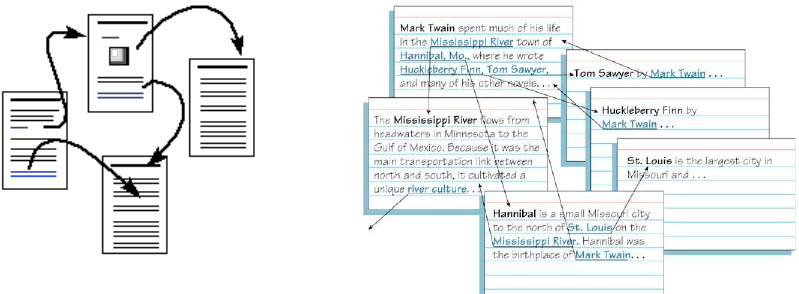
\includegraphics[scale=0.3]{figures/Schermata_20260507_103509.png}
\end{figure}


\section{Pagine Web e file HTML}
L'ipertesto prende forma concreta nella pagina Web, la quale è composta da diverse risorse (oggetti) di cui il browser deve fare il rendering, come testo, immagini o musica.

\vspace{\baselineskip}

La struttura protante e i contenuti della pagina, inclusi i riferimenti alle altre risorse, sono definiti all'interno di un file scritto in HTML (HyperText Markup Language), il linguaggio standard per la scrittura degli ipertesti.

Nel sistema, anche lo stesso file HTML è considerato a tutti gli effetti una risorsa

\newpage

\section{Meccanismi di Identificazione Univoca}
\subsection{URL - Uniform Resource Locator}
Ogni singola risorsa presente sul Web deve essere identificata in modo univoco.

Lo strumento principale per farlo è 'URL, il cui compito non è solo \textbf{identificare}, ma anche \uline{localizzare fisicamente la risorsa}, indicando in modo preciso dove andarla a trovare.

\subsubsection{Struttura dell'URL}
Un indirizzo URL si struttura unendo cinque componenti principali :
\begin{enumerate}
    \item \textbf{Nome del protocollo}

    Indica quale protocollo usare per il trasferimento dei dati
    
    \item \textbf{Indirizzo IP}

    L'indirizzo dell'host (o l'host name che andrà risolto tramite DNS)

    \item \textbf{Porta di destinazione}

    Parametro opzionale

    \item \textbf{Percorso (cammino)}

    Il percorso nell'host seguendo una gerarchia a cartelle

    \item \textbf{Identificatore della risorsa}

    Il nome del file finale
\end{enumerate}


\begin{figure}[H]
    \centering
    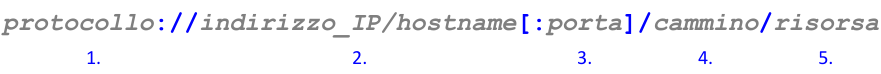
\includegraphics[scale=0.6]{figures/Schermata_20260507_105712.png}
    \caption{Struttura di un URL}
\end{figure}

\newpage

\subsection{URN - Uniform Resource Name}
Mentre l'URL indica dove si trova un oggetto, l'URN è un identificatore che definisce cosa è una risorsa, in modo del tutto indipente dalla sua posizione fisica nella rete.

Questo garantisce due proprietà essenziali :
\begin{itemize}
    \item \textbf{Persistenza}

    Il nome assegnato tramite URN rimane valido anche se la risorsa viene fisicamente spostata su un altro server

    \item \textbf{Astrazione}

    L'identificatore è slegato e non contiene alcun informazione relativa al protocollo di accesso
\end{itemize}

\subsubsection{Struttura dell'URN}
La struttura di un URN segue il formato 

\begin{enumerate}
    \item \textbf{\texttt{urn}}

    Identifica il tipo di identificatore (sempre fisso)

    \item \textbf{\texttt{<NID>} - Namespace Identifier}

    Identifica il tipo di risorsa

    \item \textbf{\texttt{<NSS>} - Namespace Specific String}

    Codice identificativo univoco della risorsa
\end{enumerate}

\begin{figure}[H]
    \centering
    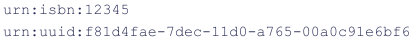
\includegraphics{figures/Schermata_20260507_110928.png}
    \caption{esempi di assegnazione identificativi univoci}

    \centering
    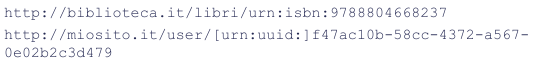
\includegraphics{figures/Schermata_20260507_111047.png}
    \caption{esempio di identificazione di una risorsa in URL}
\end{figure}


\newpage

\section{I linguaggi del Web}
All'interno dell'architettura del Web, i dati e i documenti testuali vengono espressi utilizzano una serie di linguaggi standardizzati, ognuno con uno scopo ben precisoo

\subsection{Struttura, Stile e Dati}

\subsubsection{HTML - HyperText Markup Language}
Il linguaggio fondamentale è l'\textbf{HTML}, il quale viene impiegato per \uline{definire la struttura portante e i contenuti effettivi della pagina Web.}

\subsubsection{CSS - Cascade Style Sheets}
Per gestire \textbf{l'aspetto estetico} (rendering visivo, layout e formazione), all'interno delle pagine HTML \uline{può essere integrato del codice CSS}.

\subsubsection{XML e JSON}
Quando invece l'obiettivo primario non è la visualizzazione ma la mera rappresentazione dei dati e il loro scambio tra applicazioni, si utilizzano lignuaggi standard specifici.

I più importanti e diffusi in questo ambito sono l'\textbf{XML} e il \textbf{JSON}

\subsection{Dati Multimediali e Non Testuali}
Oltre al testo, il Web è ricco di contenuti non testuali, come immagini, file audio e documenti video.

Poichè i protocolli come l'HTTP sono orientati al testo, si sfrutta la \textbf{codifica MIME}.

Questo meccanismo permette di trasformare file complessi e binari in una stringa di caratteri testuali convenzionali, rendendoli adatti a viaggiare sulla rete

\subsection{Linguaggi di scripting}
Per fare in modo che una pagina Web non sia statica ma possa offrire funzionalità avanzate e arricchire l'interazione con l'utente, essa può contenere al suo interno del codice eseguibile.

Questo codice è tipicamente espresso in linguaggi di scripting, principalmente \textbf{Javascript}

\newpage

\chapter{Protocollo HTTP - HyperText Transfer Protocol}

L'HTTP è il protocollo di livello applicativo fondamentale per il Web.

\section{Modello Client-Server}
In questo ecosistema, le responasbilità sono divise in :

\subsection{Client}
È tipicamento rappresentato da un browser web.

Il suo compito è inviare richieste e occuparsi del rendering contenuti per l'utente, un processo che può adattarsi a dispositivi diversi, inclusi quelli "non visuali".

\subsection{Server}
È il Web server, che riceve le richieste e invia gli oggetti corrispondenti in risposta. 

Un aspetto importante è che oggetti diversi che compongono una singola pagina Web possono essere prelevati anche da server Web differenti.

\section{Fase di Connessione}
L'HTTP non trasporta fisicamente i dati, ma si affida al protocollo di trasporto TCP.

La comuninicazione avviene attraverso questa procedura :

\begin{enumerate}
    \item Il client avvia una connessione TCP(creando una socket) verso l'indirizzo del server, \uline{tipicamente sulla porta 80}.
    \item Il server accetta la connessione.
    \item Client e Server si scambiano i messaggi HTTP.
    \item La connessione TCP viene chiusa.
\end{enumerate}

\section{Natura "Stateless"}
Una delle scelte architetturali più rilevanti dell'HTTP è l'essere un protocollo \textbf{stateless}, ovvero privo di stato

    \subsection{Vantaggi}
    Il server non mantiene in memoria alcuna informazione sulle richieste precedenti del client.

    Questo alleggerisce i server, evintando la complessità dei protocolli che mantengono lo stato.

    \subsection{Svantaggi}
    Ogni singola richeista deve contenere tutte le informazioni necessarie per la sua esecuzione, aumentando l'overhead.

    Per ovviare a questo limite e gestire sessioni \uline{HTTP si avvale dell'uso dei Cookie}

\section{Gestione delle Connessioni}
La gestione delle connessioni TCP fa una grande differenza sulle prestazioni e si divide in 2 approcci principali

\subsection{HTTP non persistente}
Storicamente utilizzato in \texttt{HTTP/1.0}.

Questo modello prevede che su una connessione TCP appena aperta venga inviato al massimo un solo oggetto, dopodichè la connessione viene chiusa.

Se una pagina necessita di 10 immagini, il client dovrà aprire e chiudere connessioni ripetutamente.

Il tempo di risposta per scaricare ogni singolo oggetto è pari a \textbf{\texttt{2 RTT (Round Trip Time) + il tempo di trasmissione dell'oggetto}}

\subsection{HTTP persistente}
Adottato da \texttt{HTTP/1.1, HTTP/2.0 e HTTP/3.0} questo modello lascia la connessione aperta.

Sfruttano un'unica connessione, \uline{il server può inviare al client più oggetti in sequenza}.

In condizione in cui l'\texttt{RTT} è molto maggiore del tempo di trasmissione, questo approccio dimezza all'incirca i tempi di caricamento per ogni risorsa successiva alla prima.

\newpage

\section{Struttura e Formato dei Messaggi}
HTTP  è un protocollo orientato al carattere, di conseguenza, il formato dei suoi messaggi si basa su testo leggibile (\texttt{ASCII}).

\subsection{Formato delle Richieste}

    \begin{center}
        \begin{tcolorbox}[title=Esempio messaggio di richiesta]
        \ttfamily
        GET /index.html HTTP/1.1\textbackslash 
        Host: www-net.cs.umass.edu\textbackslash r\textbackslash n \\
        User-Agent: Mozilla/5.0 (Macintosh; Intel Mac OS X 10.15; rv:80.0) Gecko/20100101 Firefox/80.0 \textbackslash r\textbackslash n \\
        Accept: text/html,application/xhtml+xml\textbackslash r\textbackslash n \\
        Accept-Language: en-us,en;q=0.5\textbackslash r\textbackslash n \\
        Accept-Encoding: gzip,deflate\textbackslash r\textbackslash n \\
        Connection: keep-alive\textbackslash r\textbackslash n
    \end{tcolorbox}
    \end{center}

\subsubsection{Caratteri speciali}
Ogni messaggio di richiesta è strutturato in una sequenza precisa di righe separate tra loro tramite due speciali caratteri di controllo
    
    \begin{itemize}
        \item \textbf{\texttt{cr-carriage return} (ritorno a capo)}
        \item \textbf{\texttt{lf-line feed} (nuova linea)}
    \end{itemize}

\subsubsection{Riga di richiesta}
È la riga di apertura del messaggio.

Contiene 3 parametri separati da uno spazio (\texttt{sp})

    \begin{itemize}
        \item Il \textbf{metodo} \texttt{HTTP} che il client vuole eseguire
        \item L'\textbf{\texttt{URL}} identificativo della risorsa
        \item La \textbf{versione} del protocollo \texttt{HTTP} in uso
    \end{itemize}

    \begin{center}
        \begin{tcolorbox}[title=Esempio: Riga di richiesta]
            \texttt{GET /index.html HTTP/1.1\textbackslash r\textbackslash n}
        \end{tcolorbox}
    \end{center}

\subsubsection{Righe di intestazione}
Subito dopo la riga di richiesta, si collocano gli header.

Sono  strutturati nel formato \textbf{\texttt{nome-campo: valore}} e seguiti da un \textbf{\texttt{cr lf}}.

Servono al client per passare vari parametri al server, come ad esempio : 

    \begin{itemize}
        \item \textbf{Host} 
        
        L'host specifico in cui risiede l'oggetto
        \item \textbf{User-Agent} 
        
        Il tipo di browser in uso
        \item \textbf{Accept}
        
        Preferenze sulla negoaziazione del contenuto tramite formati \texttt{MIME}
        \item \textbf{Preferenze aggiuntive}
        Come la lingua (\texttt{Accept-Language}) o il tipo di compressione accettata \texttt{(Accept-Encoding)}
    \end{itemize}

    
    \begin{center}
        \begin{tcolorbox}[title=Esempio Righe di intestazione]
            \ttfamily
            Host: www-net.cs.umass.edu\textbackslash r\textbackslash n \\
            User-Agent: Mozilla/5.0 (Macintosh; Intel Mac OS X 10.15; rv:80.0) Gecko/20100101 Firefox/80.0 \textbackslash r\textbackslash n \\
            Accept: text/html,application/xhtml+xml\textbackslash r\textbackslash n \\
            Accept-Language: en-us,en;q=0.5\textbackslash r\textbackslash n \\
            Accept-Encoding: gzip,deflate\textbackslash r\textbackslash n \\
            Connection: keep-alive\textbackslash r\textbackslash n
        \end{tcolorbox}
    \end{center}
        

\subsection{Formato delle Risposte}
I messaggi restituiti dal server iniziano con una riga di stato, seguita dalle righe di intestazione e infine dai dati effettivi (come il file HTML o l'immagine richiesta)

    \begin{figure}[H]
        \centering
        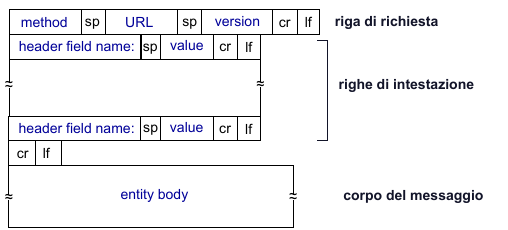
\includegraphics{figures/Schermata_20260507_160135.png}
        \caption{Struttura del messagio generale}
    \end{figure}

\newpage

\section{Metodi HTTP}
I metodi HTTP definiscono l'azione specifica che il client desidera effettuare sulla risorsa indicata dall'URL.

Prima di elencarli è essenziale comprendere 2 parametri fondamentali con cui questi metodi vengono classificati

\subsection{Le proprietà dei metodi}
I metodi si distinguono in base a 2 proprietà che descrivono il loro impatto sui dati presenti nel server

\subsubsection{Metodi Sicuri}
Un metodo viene definitio sicuro se \uline{la sua esecuzione non modifica in alcun modo lo stato del server}.

Serve, in sostanza solo per la lettura

\subsubsection{Metodi Idempotenti}
Un metodo è considerato idempotente quando l'efffetto che ha sul server dopo una singola richiesta andata a buon fine   \uline{è esattamente identico all'effetto che si otterrebbe eseguendo più richieste identiche in modo consecutivo.}

\subsection{Metodo GET}
Il metodo \texttt{GET} richiede al server di recuperare la risorsa specifica dall'\texttt{URL} o qualunque informazione a essa relativa.

È il metodo più comune per ottenere dati in vari formati, come docomenti \texttt{HTML, XML, JSON} o contenuti multimediali.

Se la richiesta necessità di parametri, questi vengono agganciati direttamente in coda all'\texttt{URL}.

\subsubsection{Proprietà}
Trattandosi di un metodo di sola lettura, la \texttt{GET} è classificata come metodo \textbf{sicuro} e \textbf{idempotente}.

\subsection{Metodo HEAD}
La \texttt{HEAD} è praticamente identica alla \texttt{GET}, ma con una differenza cruciale : \uline{il server non deve restituire il corpo del messaggio nella risposta}, ma solo le righe di intestazione.

L'uso tipico di questo metodo è il \textbf{debugging} oppure l'ottenimento di informazioni meta-dati su una risorsa

\subsubsection{Proprietà}
Esattamente come la \texttt{GET}, anche la \texttt{HEAD} è un metodo \textbf{sicuro} e \textbf{idempotente}.

\begin{tcolorbox}[title=Esempio di GET]
    \texttt{GET myCompany/orders?item="Q2345"\&date="2022/03" HTTP1.1}
\end{tcolorbox}

\subsection{Metodo OPTIONS}
Questo metodo rappresenta una richiesta per ottenere \uline{informazioni sulle opzioni di comunicazione} permesse relativamente alla risorsa identificata dall'\texttt{URL}.

\subsubsection{Proprietà}
È un metodo \textbf{sicuro} e \textbf{idempotente}.

\subsection{Metodo TRACE}
Viene utilizzato per invocare un \uline{loopback del messaggio di richiesta} a livello applicativo da parte del server, utile anch'esso per scopi diagnostici.

\subsubsection{Proprietà}
È un metodo \textbf{sicuro} e \textbf{idempotente}.

\subsection{Metodo POST}
La \texttt{POST} viene utilizzata per \uline{comunicare al server dei dati che devono essere elaborati}, o per richiedere che il server accetti la risorsa inclusa nella richiesta come un nuovo "subordinato dall'\texttt{URL} indicato.

A differenza della \texttt{GET}, i dati non vengono passati nell'\texttt{URL}, ma sono \uline{inseriti come documento autonomo all'interno del corpo della richiesta}, subito dopo le righe di intestazione.

L'uso tipico è trasportare i dati compilati da un utente all'interno di un form.

\subsubsection{Proprietà}
Poichè la \texttt{POST} serve tipicamente a creare o aggiornare dati sul server, \textbf{non è un metodo sicuro e non è idempotente}.

\begin{tcolorbox}[title=Esempio di POST]
\ttfamily
POST myCompany/orders HTTP1.1 \\
Content-Length: 59 \\
Content-Type: application/x-www-form-urlencoded \\
update=true\&oldItem="Q2345"\&newItem="Q68254"\&date="2022/04"
\end{tcolorbox}

\subsection{Metodo PUT}
La \texttt{PUT} richiede che la risorsa fornita venga memorizzata e \uline{caricata sul server all'\texttt{URL} specificato}.

La sua particolarità è che, se nell'URL indicato esiste già un file, questo \textbf{viene completamente sostituito} dal nuovo contenuto presente nel corpo della richiesta.

\subsubsection{Proprietà}
Modificando i file, la \texttt{PUT} non è un metodo sicuro.

Tuttavia a differenza della \texttt{POST}, \textbf{è un metodo idempotente} : caricare o sovrascrivere lo stesso file una volta oppure cento volte porta sempre all'identico stato finale sul server

\subsection{Metodo DELETE}
Come deducibile dal nome, questo metodo richiede esplicitamente al server di \textbf{eliminare la risorsa} identificata dall'\texttt{URL}.

\subsubsection{Proprietà}
Non essendo un'operazione di sola lettura, non è un metodo sicuro.

Tuttavia, \textbf{è un metodo idempotente}: richiedere l'eliminazione di un file già eliminato non comporta ulteriori cambiamenti di stato nel server.

\section{Codici di stato}
I codici di stato sono valori numerici, accompagnati da una breve descrizione testuale, restituiti dal Web server al client all'interno dei messaggi di risposta \texttt{HTTP}.

La loro funzione è comunicare l'esito dell'operazione richiesta.

Fisicamente, si trovano nella riga di stato, ovvero la primissima riga del messaggio di risposta inviato dal server

\subsection{Le 5 classi dei codici di stato}
I codici sono suddivisi rigorosamente in 5 diverse classi, categorizzate in base al 1° numero della cifra.

\subsubsection{\texttt{1xx} (Informational)}
I codici che iniziano con 1 indicano una comunicazione di tipo informativo.

Segnalano al client che la richiesta è stata ricevuta e che il server sta continuando regolarmente la sua elaborazione.

\subsubsection{\texttt{2xx} (Success)}
I codici che iniziano con 2 vengono utilizzati per confermare un successo.

Indica che la richiesta del client è stata correttamente ricevuta, compresa, accettata ed elaborata dal server.

\subsubsection{\texttt{3xx} (Redirection)}
Questa classe di codici segnala che la risorsa non può essere fornita direttamente, ma che è necessario che il client intraprenda ulteriori azioni per poter completare la richiesta in modo corretto.

\subsubsection{\texttt{4xx} (Client Error)}
I codici \texttt{4xx} indicano che il problema è imputabile a chi ha fatto la richiesta.

Segnalano che la richiesta inviata dal client presenta una sintassi errata oppure risulta incomprensibile al server.

\subsubsection{\texttt{5xx} (Server Error)}
I codici \texttt{5xx} indicano un errore imputabile all'infrastruttura di destinazione.

Segnalano che il server non è riuscito a soddisfare una richiesta che risultava apparentemente valida.

\section{I Cookie e il mantenimento dello stato}
Per risolvere il limite imposto dall'assenza di stato, \uline{i client e i server \texttt{HTTP} si avvalgono dei cookie per riuscire a mantenere in memoria lo stato nelle transizioni}.

Questa tecnologia viene impiegata tipicamente per 3 scopi principali:

\begin{enumerate}
    \item Gestione dell'autorizzazione e autenticazione
    \item Mantenimento del carrello negli acquisti online
    \item Creazione di raccomandazioni (come ad esempio le pubblicità mirate)
\end{enumerate}

\subsection{L'architettura dei Cookie}
L'intero meccanismo di funzionamente dei cookie si basa su 4 componenti fondamentali che lavorano in sinergia: 

\begin{enumerate}
    \item Una \textbf{riga di intestazione specifica presente nella risposta \texttt{HTTP}} generata dal server
    \item Una \textbf{riga di intestazione specifica inserita nella successiva richiesta \texttt{HTTP}} da parte del client.
    \item Un \textbf{file locale relativo al cookie}, conservato sul dispositivo del client e gestito dal suo browser.
    \item Un \textbf{database di backend} mantenuto e gestito attivamente dal Web server
\end{enumerate}

\section{Web Caching}
L'obiettivo principale del Web caching è \uline{soddisfare le richieste dei client utilizzando delle copie salvate localmente}, invece di dover scaricare i file dal server Web di origine.

Questo copie possono risiedere in 2 posti:

\begin{enumerate}
    \item Nella \textbf{Web cache locale del dispositivo}, gestita direttamente dal browser dell'utente
    \item In appositi server disseminati nelle reti istituzionali o di accesso, noti come \textbf{Web cache} o \textbf{server proxy}
\end{enumerate}

\subsection{Il ruolo del Server Proxy}
Quando un proxy è attivato, il browser invia tutte le sue richieste \texttt{HTTP} direttamente a questo nodo intermedio.

Il server proxy svolge un doppio ruolo:

\begin{itemize}
    \item \textbf{Si comporta da Server}

    Se possiede già in memoria l'oggetto richeisto dal client, lo invia immediatamente

    \item \textbf{Si comporta da Client}

    Se l'oggetto non è presente nella sua cache, lo richiede al server Web di origine, lo salva e infine lo inoltra al client che lo aveva richiesto
\end{itemize}

È il server di origine a dettare le regole alla cache: attraverso intestazioni specifiche nella risposta \texttt{HTTP}, comunica se un file può essere salvato e per quanto tempo

\section{GET condizionale}
Il problema principale delle cache è capire se il file salvato in memoria è ancora la versione più recente, oppure se il server di origine lo ha oggiornato.

Per risolvere questo problema, il protocollo \texttt{HTTP} utilizza una richiesta speciale detta "\texttt{GET} condizionale".

\subsection{L'intestazione "\texttt{if-modified-since"}}
Quando il client (o il proxy) richiede un file che ha già in cache ma di cui vuole verificare la validità, inserisce nella richiesta \texttt{HTTP} un parametro specifico: \texttt{if-modified-since: <data>}

Con questa riga, il client sta dicendo al server: 

"Inviami questo file solo se è stato modificato dopo questa precisa data (ovvero la data in cui ho scaricato la mia copia locale)"

\subsubsection{Possibili risposte del Server}
A fronte di una \texttt{GET} condizionale, il server Web controlla il file originale e può rispondere in due modi:

\begin{itemize}
    \item \textbf{Se il file NON è stato modificato}
    
    Il server genera un messaggio di risposta con il codice di stato \texttt{304 Not Modified}.

    La particolarià fondamentale è che \textbf{questa risposta è vuota}, ovvero non include alcun oggetto al suo interno.

    Questo permette di risparmiare un'enorme quantità di banda e tempo di trasferimento, autorizzando il client a usare la copia che ha già in memoria.

    \item  \textbf{Se il file È stato modificato}
    
    Il server elabora la richiesta come una normale \texttt{GET}.

    Risponde con un codice \texttt{200 OK} e inserisce nel corpo del messaggio la nuova versione aggiornata dei dati.
\end{itemize}

\newpage

\section{Message vs Streaming communication}
La differenza principale tra la comunicazione a messaggi e quella a stream risiede nel modo in cui i dati vengono elaborati e percepiti dai diversi livelli dell'architettura di rete

\subsection{Livello di Applicazione (Comunicazione a Messaggi)}
A livello applicativo, come nel caso del protocollo \texttt{HTTP}, la comunicazione è \textbf{orientata al messaggio}.

Questo significa che i software comunicano scambiandosi pacchetti di dati interi e ben definiti (i messaggi).

\subsection{Livello di Trasporto (Comunicazione a Stream e Segmenti)}
Per il livello di trasporto, i messaggi non esistono come entità logiche, ma sono visti nel loro complesso come un \textbf{flusso di byte da trasportare in rete}.

Il livello di trasporto prende questo stream e lo scompone in \textbf{segmenti}.

La gestione di questi segmenti dipende dal protocollo utilizzato:

\begin{itemize}
    \item \textbf{Servizio UDP}

    Il protocollo scompone lo stream di byte in segmenti e li inoltra al livello di rete in \textbf{modalità best-effort}

    \item \textbf{Servizio TCP}

    Anche il TCP scompone e invia lo stream come segmenti, ma \textbf{ogni segmento viene numerato}.

    Questa numerazione permette a TCP di garantire 3 funzionalità cruciali:
    \begin{enumerate}
        \item \textbf{Riordinamento}

        I segmenti arrivati fuori sequenza vengono rimessi in ordine giusto.

        \item \textbf{Controllo delle duplicazioni}

        I segmenti ricevuti più volte vengono scartati

        \item \textbf{Controllo delle perdite}

        Il sistema si accorge dei buchi nella numerazione e richiede il rinvio dei segmneti mancanti
    \end{enumerate}
\end{itemize}

\newpage

\section{Tipi di comunicazione Message-oriented communication}
La differenza fondamentale tra i vari tipi di comunicazione si basa sul \textbf{punto di sincronizzazione}, ovvero il momento esatto in cui il client smette di attendere una conferma e riprende regolarmente la propria esecuzione.

\subsection{Comunicazione Persistente Asincrona}
\begin{itemize}
    \item \textbf{Punto di sincronizzazione}

    Avviene all'\textbf{invio della richiesta}

    \item \textbf{Funzionamento}

    Il mittente sospende la sua esecuzione solo per il tempo necessario affinchè il messaggio venga preso in carico dal proprio sistemo intermedio locale (il middleware lato mittente), e non attende alcuna risposta dal destinatario finale

    \item \textbf{Esempio}

    Il classico sistema di posta elettronica, in cui il client attende solo che il proprio server \texttt{SMTP} accetti l'email da spedire.
\end{itemize}

\subsection{Comunicazione persistente sincrona}
\begin{itemize}
    \item \textbf{Punto di sincronizzazione}

    Avviene all'inoltro della richiesta

    \item \textbf{Funzionamento}

    Il mittente invia il messaggio e attende.

    Riprenderà la sua esecuzione solo quando il software middleware situato fisicamente sul lato del ricevente avrà ricevuto il messaggio e avrà inviato una notifica di avvenuta consegna.
\end{itemize}

\subsection{Comunicazione transiente sincrona basata sulla consegna (Delivery based)}
\begin{itemize}
    \item \textbf{Punto di sincronizzazione}

    Avviene all'inizio dell'\textbf{elaborazione della richiesta}(at request processing)

    \item \textbf{Funzionamento}

    Il mittente rimane bloccato in attesa finchè l'applicazione destinataria (che deve essere attiva) gli notifica di aver effettivamente iniziato a elaborare la richiesta ricevuta.

    \item \textbf{Esempio}

    L'invio di comandi a un server remoto tramite protocollo \texttt{SSH}
\end{itemize}

\subsection{Comunicazione transiente sincrona basata sulla risposta (Response based)}
\begin{itemize}
    \item \textbf{Punto di sincronizzazione}

    Avviene \uline{dopo l'elaborazione della richiesta (after processing)}

    \item \textbf{Funzionamento}

    È il modello che richiede l'attesa maggiore.

    Il mittente rimane in sospeso e continua l'esecuzione solo quando il destinatario ha elaborato con successo e in modo completo la richiesta, restituendo la risposta finale.

    \item \textbf{Esempio}

    Il protocollo \texttt{HTTP} in cui il browser attende di ricevere dal server la risorsa richiesta.
\end{itemize}

\section{Modello a Code di Messaggi (Message Queuing)}
In questo modello, le applicazioni non comunicano passandosi i dati direttamente, ma \uline{inseriscono i messaggi all'interno di code specifiche} gestite da appositi gestori (queue manager)

Questa architettura si basa su 2 caratteristiche fondamentali:
\begin{itemize}
    \item \textbf{Persistenza (Storage)}

    Il sistema ha la capacità di memorizzare fisicamente i messaggi.

    Una volta che un messaggio viene inserito all'interno di una coda, vi rimane al sicuro finchè non viene esplicitamente prelevato e rimosso.

    \item \textbf{Disaccoppiamento temporale (Asincronismo)}

    Non è assolutamente necessario che il mittente e il destinatario siano in esecuzione nello stesso momento.

    Il mittente può generare un messaggio che se il ricevente è spento e, viceversa, il ricevente può recuperarlo dalla sua coda molto tempo dopo che il mittente ha finito di lavorare
\end{itemize}

\subsection{Operazioni per interagire con la coda}
Per interagire con queste code, l'interfaccia di comunicazione fornisce \textbf{4 primitive di base}.

\begin{enumerate}
    \item \textbf{\texttt{PUT}}

    Inserisce un messaggio nella coda di invio (operazione non bloccante).
    \item \textbf{\texttt{GET}}

    Rimuove il primo messaggio disponibile dalla coda di ricezione (operazione bloccante, il ricevente si ferma ad aspettare finchè non arriva un messaggio).
    \item \textbf{\texttt{POLL}}

    Controlla in modo non bloccante la presenza di messaggi e, se ci sono, rimuove il primo.
    \item \textbf{\texttt{NOTIFY}}

    Installa un "handler" (una funzione di callback) che viene richiamato automaticamente dal middleware non appena un nuovo messaggio inserito nella codam avvisando l'applicazione.
\end{enumerate}

\newpage

\section{Message Broker e Pattern Publish/Subscribe}
Il pattern Publish/Subscribe è un evoluzione che utilizza un nodo centrale chiamato \textbf{Message Broker} per gestire lo smistamento delle informazioni, basandosi sugli \textbf{argomenti} (Topic) anzichè sugli indirizzi di destinazione.

L'architettura funziona in questo modo:
\begin{itemize}
    \item \textbf{I Publisher (pubblicatori)}

    Non sanno chi riceverà i loro dati, si limitano a collegarsi al broker dichiarando:

    "voglio inviare messaggi relativi a questo specifico Topic".

    \item \textbf{I Subscriber (sottoscrittori)}

    A loro volta, si registrano al broker dichiarando:

    "voglio ricevere tutti i messaggi pubblicati su questo Topic".
\end{itemize}

Questa meccanica garantisce una \textbf{totale indipendenza} tra chi produce i dati e chi li consuma, rendendo facilissimo creare reti di comunicazione complesse del tipo uno-a-motli, molti-a-uno o molti-a-molti.

Se per un certo topic non ci sono subscriber attivi in quel momento, il broker può mantenere i dati in memoria applicando diverse politiche.

\subsection{Funzionalità speciali per i sistemi critici (es. protocollo \texttt{MQTT})}
Poichè il modello pub/sub è massicciamente utilizzato nell'Internet of things e in ambienti critici, i broker offrono funzionalità avanzate:
\begin{itemize}
    \item \textbf{Messaggio "Retain"}

    Il publisher può chiedere al broker di conservare uno e un solo messaggio per un topic.

    Grazie al flag retain, non appena un nuovo subscriver si connette, riceve immediatamente quest'ultimo valore valido senza dover aspettare una nuova pubblicazione.

    \item \textbf{Last Will and Testament (LWT)}

    Al momento della connessione, il publisher può consegnare al broker un "testamento".

    Se il dispositivo publisher dovesse subire una disconnessione inaspettata, il broker inoltrerà automaticamente questo messaggio di allarme a tutti i subscriber.

    È una funzione fondamentale per accorgersi tempestivamente di un'anomalia nei sistemi critici.
\end{itemize}